\chapter{Drahtlose Datenübertragung}

Der Bedarf an drahtlosen Technologien im industriellen sowie im privaten Umfeld steigt immer mehr. Die Schlüsselfaktoren, die hinter den Anforderungen für drahtlose Technologien stehen, sind zum einen die Fernsteuerung, damit verbunden die Mobilität und Flexibilität, zum anderen die verlustlose Übertragung von Daten. Beispielsweise können drahtlose Sensoren und Aktoren, die auf beweglichen Teilen von Maschinen positioniert werden, von Vorteil für drahtlose Systeme sein. Jede Anwendung hat unterschiedliche Anforderungen. Es gibt kein einzelnes drahtloses System, das alle Anforderungen gleichzeitig erfüllen kann.\\
Im Rahmen dieser Arbeit wurden mehrere Funktechnologien, die im \acrshort{iot}-Umfeld in Frage kommen angeschaut und deren Vor- und Nachteile aufgezeigt..

\section{\acrshort{ble}}

Ursprünglich wurde \acrfull{ble} als \glqq{}Bluetooth 4.0\grqq{} bezeichnet, als es im Jahre 2011 auf den Markt kam. Doch die Ausrichtung auf geringen Energieverbrauch, was der Hauptvorteil gegenüber dem regulären Bluetooth Standard ist, war marketingtechnisch so wichtig, dass sich dies auch im Namen manifestieren musste. Laut eigenen Angaben kann eine einzelne Batterie ein Produkt, das über \acrshort{ble} verbunden ist, bis zu fünf Jahren betreiben kann, ist diese Technologie ideal für \acrshort{m2m}-Kommunikation.

\acrshort{ble} operiert im 2.4 GHz \gls{ism}, wie Bluetooth 1.0. Doch um Energie zu sparen, wurde die Übertragungszeit auf wenige Millisekunden, dafür aber mit einer hohen Datenrate von 1 Mbs optimiert. Danach geht \acrshort{ble} sofort in einen Schlafmodus bis wieder eine Verbindung aufgebaut wird.
Durch die begrenzte Reichweite von etwa 100m (Sichtverbindung) eignet sich \acrshort{ble} vor allem für Anwendungen im nahen Umkreis wie kontaktloses Zahlen, Dienste im öffentlichen Verkehr oder Aufzeichnen des Gesundheitszustands und Fitness.

\section{\gls{zigbee}}

\gls{zigbee} ist ein Mesh-Netzwerk Protokoll. Es ist dafür ausgelegt kleine Datenpakete über kurze Distanzen zu Übertragen und dabei möglichst wenig Energie zu verbrauchen. In einer Mesh-Topologie werden Daten eines einzelnen Sensors durch ein Netz von \gls{iotk} geleitet. Jeder \gls{iotk} fungiert dabei gleichzeitig als Datenquelle und Übermittler (Repeater) bis die Daten den \gls{iotg} erreicht haben.

\gls{zigbee} verwendet eine Version des \gls{ieee802.15.4} Standards und ist deshalb in lokalen Sensor Netzwerken, vor allem in der Gebäude Automation weit verbreitet. \gls{zigbee} verwendet das 2.4 GHz \gls{ism} und kann, weil dies ein internationaler Standard ist, praktisch überall auf der Welt eingesetzt werden.

\section{\gls{3gpp}}

\gls{3gpp} - Die Industrie Experten hinter der Standardisierung von Zellulären Netzwerken - haben kürzlich drei neue Standards vorgestellt:

\begin{enumerate}
  \item LTE-MTC (auch bekannt unter LTE-M)
  \item NB-LTE-M
  \item NB-IoT
\end{enumerate}

Dies sind die Bestrebungen der Telekommunikationsbranche Geräte die in einem Träger Netzwerk operieren günstiger und energieeffizienter zu machen, nicht zuletzt um Einfluss auf das Internet der Dinge (LTE \acrshort{iot}) und die \acrfull{m2m} Kommunikation zu gewinnen. Diese neuen Standards sind eine Antwort auf \gls{lora}, \gls{lorawan} und \gls{sigfox}, also die \gls{lpwan}-Technologien.

\subsection{LTE-MTC (LTE-M)}

LTE-M, eine abgekürzte Version von LTE-MTC (Machine-Type Communications) ist Teil von \gls{3gpp}'s Release 12 und 13 und ist immer noch in der Evaluationsphase. Der \gls{lte} Kanal besteht aus Ressource-Blöcken die je etwa 230 kHz des Frequenzspektrums besetzten. LTE-M ist Teil des 1.4 MHz Blocks, der aus sechs Ressource-Blöcken besteht. LTE-M ist aufgrund seines erweiterten, diskontinuierlichen Repetitionszykluses (DRX) energieeffizienter. Dies bedeutet, dass ein Endgerät mit der Basis Station vereinbaren kann, wie oft es aufwacht um Daten zu Empfangen.\\
Der Vorteil von LTE-MTC für \acrshort{m2m} Kommunikation ist, dass es sich in das bestehende Konstrukt von \gls{lte} Netzwerken eingliedert. In anderen Worten, der Netzwerk Provider muss nur seine Basisband-Software auf seinen Basis Stationen aktualisieren und muss keine Geld für neue Antennen ausgeben. Die Empfänger sind auch viel einfacher aufgebaut als z.B. ein Smartphone, denn sie müssen nur 1.4 MHz digitalisieren können, anstatt 20 MHz.\\
LTE-M hat eine leicht höhere Datenrate als NB-LTE und NB-IoT, es können relativ grosse Datenmengen übertragen werden. Darum ist LTE-M für Anwendungen wie Object Tracking, Wearables, Energiemanagement und Stadt-Infrastruktur geeignet. 

\subsection{NB-LTE-M}

Wie LTE-M ist NB-LTE-M ein anderer Overlay der existierenden LTE Struktur. Dabei werden bestehende Ressource-Blöcke für \gls{iot} Datenverkehr reserviert und kleinere Kanäle verwendet um einfachere Empfänger bauen zu können. NB-LTE-M schlägt die Wiederverwendung von GSM vor, indem ein einzelner ~200 kHz Ressource-Block verwendet wird.\\
Was NB-LTE-M einzigartig macht, ist, dass es nur einen LTE Ressource-Blöck verwendet, anstatt das 1.4 MHz Spektrum und sechs Ressource-Blöcke. Dies ergibt für den Endbenutzer einen effektiven Durchsatz von etwa 200 kb/s down und 144 kb/s up.

\subsection{NB-IoT}

NB-IoT ist ein anderer \gls{3gpp}-Release 13 Vorschlag der nicht auf LTE, sondern auf einer DSSS (Direct Sequence Spread Spectrum) Modulation basiert. Die Komplexität um Endgeräte dafür zu bauen ist noch geringer als bei NB-LTE-M und zusätzlich können auch kostengünstigere Chipsets verwendet werden. Befürworter von NB-IoT, wie Huawei, Ericsson, Qualcomm, und Vodafone, arbeiten aktiv zusammen um diesen Standard durchzusetzen.\\
Die Schwierigkeit von NB-IoT ist die Verbreitung der Infrastruktur. Da es nicht Teil des LTE Standards ist, muss es entweder in einem Nebenband operieren, was die Netzwerkanbieter viel Geld kosten kann, oder es muss das veraltete GSM Spektrum wiederverwenden.

\section{\gls{wlan}}

\gls{wlan} ist ein Drahtloses lokales Netzwerk das im \gls{ieee802.11} Standard spezifiziert ist. \gls{wlan} wird hauptsächlich verwendet um Computer, Laptops, Tablets, Smartphones, etc. über einen Internet Gatway, meist in Form eines Access Points, mit dem Internet zu verbinden. Grundsätzlich können aber beliebige zwei Hardware Komponenten miteinander verbunden werden.\\
\gls{wlan} unterstützt zwei \glspl{ism}; das globale 2.4 GHz UHF ISM und das 5 GHz SHF Radioband. Die WiFi Allianz zertifiziert einige Produkte, die dann mit dem \glqq{}Wi-Fi Certified\grqq{} bezeichnet werden dürfen. Um dieses Zertifikat zu erhalten, muss das Produkt den Interoperabilitäts-Tests der Allianz genügen. Somit ist die Integration von \gls{wlan} in ein neues oder bereits bestehendes System sehr einfach, da \gls{wlan} weit verbreitet ist. Weiter sind auch die maximal erreichbaren Datenraten beachtlich, Router der neusten Generation erreichen Datenraten von über 900Mbps mit dem \gls{ieee802.11}ac Standard auf dem 5 GHz Band.\\
Doch für den Einsatz in einer \gls{iot} Umgebung überwiegen meist die Nachteile. \gls{wlan} Transmitter verbrauchen viel Energie, ein mehrwöchiger batteriebetriebener Einsatz in einem \gls{iotk} ist nicht realistisch. Durch die hohe Datenrate ist gleichzeitig die Reichweite sehr beschränkt. Je nach Umgebung meist nur etwa 100m.

\section{\gls{sigfox}}

\gls{sigfox} ist eine Ultra-Schmalband-Technologie die von der gleichnamigen Firma entwickelt wird. Das Unternehmen baut eine eigene Netzinfrastruktur mit Partnern auf und vermietet diese dann als Service inklusive Cloud Plattform. Wie bei Telekom-Anbietern wird die Abdeckung durch Funkantennen gewährleistet und ist bereits in 20 Ländern verfügbar.\\
\gls{sigfox} verwendet unlizenzierte \glspl{ism}; 868 MHz in Europa und 902 MHz in den USA. 
\gls{sigfox} nutzt die Standard Modulationsverfahren BPSK (Binary Phase-Shift Keying) für den Uplink und GFSK (Gaussian Frequency-Shift Keying) für den Downlink. Dabei verwendet \gls{sigfox} ganz kleine Teile des Frequenzspektrums und ändert die Phase der Trägerradiowelle um die Daten zu encodieren. Dies erlaubt dem Empfänger nur auf einem ganz kleinen Abschnitt des Spektrums zu hören, was den Effekt des Rauschens abschwächt.
Da \gls{sigfox} als Service angeboten wird, muss, wer diese Technologie verwenden will, die Daten in die Cloud von SigFox laden und auch entsprechend dafür bezahlen. Traffic und Grösse sind dabei aber stark begrenzt:

\begin{itemize}
  \item bis zu 140 Nachrichten pro \gls{iotk} pro Tag
  \item Payload Grösse von 12 Byte für jede Nachricht
  \item Datendurchsatz von bis zu 100 bit pro Sekunde
\end{itemize}

Mit einer Sensitivität von 129 dB kann über sehr weite Strecken gefunkt werden. In ländlichen Gebieten soll die Reichweite 30-50 km betragen, in urbaneren Gebieten durch diverse Hindernisse und höherem Rauschen nur noch zwischen 3 und 10 km. \\
Während die Endpunkt-Geräte sehr simpel und dadurch auch kostengünstig sind, werden dafür besser ausgestattete Basis Stationen benötigt. Die \gls{sigfox} Kommunikation funktioniert tendenziell besser von den Endpunkten zur Basistation. Bidirektionale Kommunikation wird zwar unterstützt, aber die Kapazität von der Basis Station zurück zum Endpunkt ist beschränkt und auch das Downlink Budget ist geringer. Dies ist auf die geringere Empfangssensitivität des Endpunkts gegenüber der teuren Basis Station zurückzuführen.

\section{\gls{lora}}

\gls{lora} ist eine Modulationstechnologie um den Kommunikationslink über weite Strecken aufzubauen. Viele veraltete Drahtlossysteme nutzen das FSK (Frequency-Shift Keying) Modulationsverfahren, weil es sehr energieeffizient ist. \gls{lora} basiert auf dem CSS (Chirp Spread Spectrum) Modulationsverfahren, welches die gleichen energieeffizienten Charakteristiken aufweist, aber gleichzeitig die Reichweite massiv erweitert und zudem auch robuster gegen Interferenz ist. CSS ist beim Militär und zur Kommunikation im Weltraum schon seit Jahrzehnten im Einsatz, gerade wegen den langen Kommunikationsdistanzen, die erreicht werden können. \gls{lora} ist die erste kostengünstige Implementation für den kommerziellen Einsatz.    

Der Vorteil von \gls{lora} ist die auf weite Distanzen ausgelegte Technologie. Ein einzelnes Gateway oder Basis Station kann ganze Städte oder hunderte Quadratkilometer abdecken. Die Reichweite ist stark von der Umgebung und der sich in ihr befindenden Hindernissen abhängig. Aber \gls{lora} besitzt eine sehr hohe Sensitivität, je nach Modul bis zu -148 dBm. 

\section{\gls{lorawan}}

\gls{lorawan} ist der MAC-Layer für \gls{lora} und definiert damit die Sicherungsschicht. Das Protokoll und die Systemarchitektur haben einen grossen Einfluss auf die Batterielaufzeit eines \gls{iotk}. Die Netzwerkkapazität hat Einfluss auf die Servicequalität, die Sicherheit und die Vielfältigkeit der Anwendungen die das Netzwerk unterstützt.

\begin{figure}[H]
     \centering
        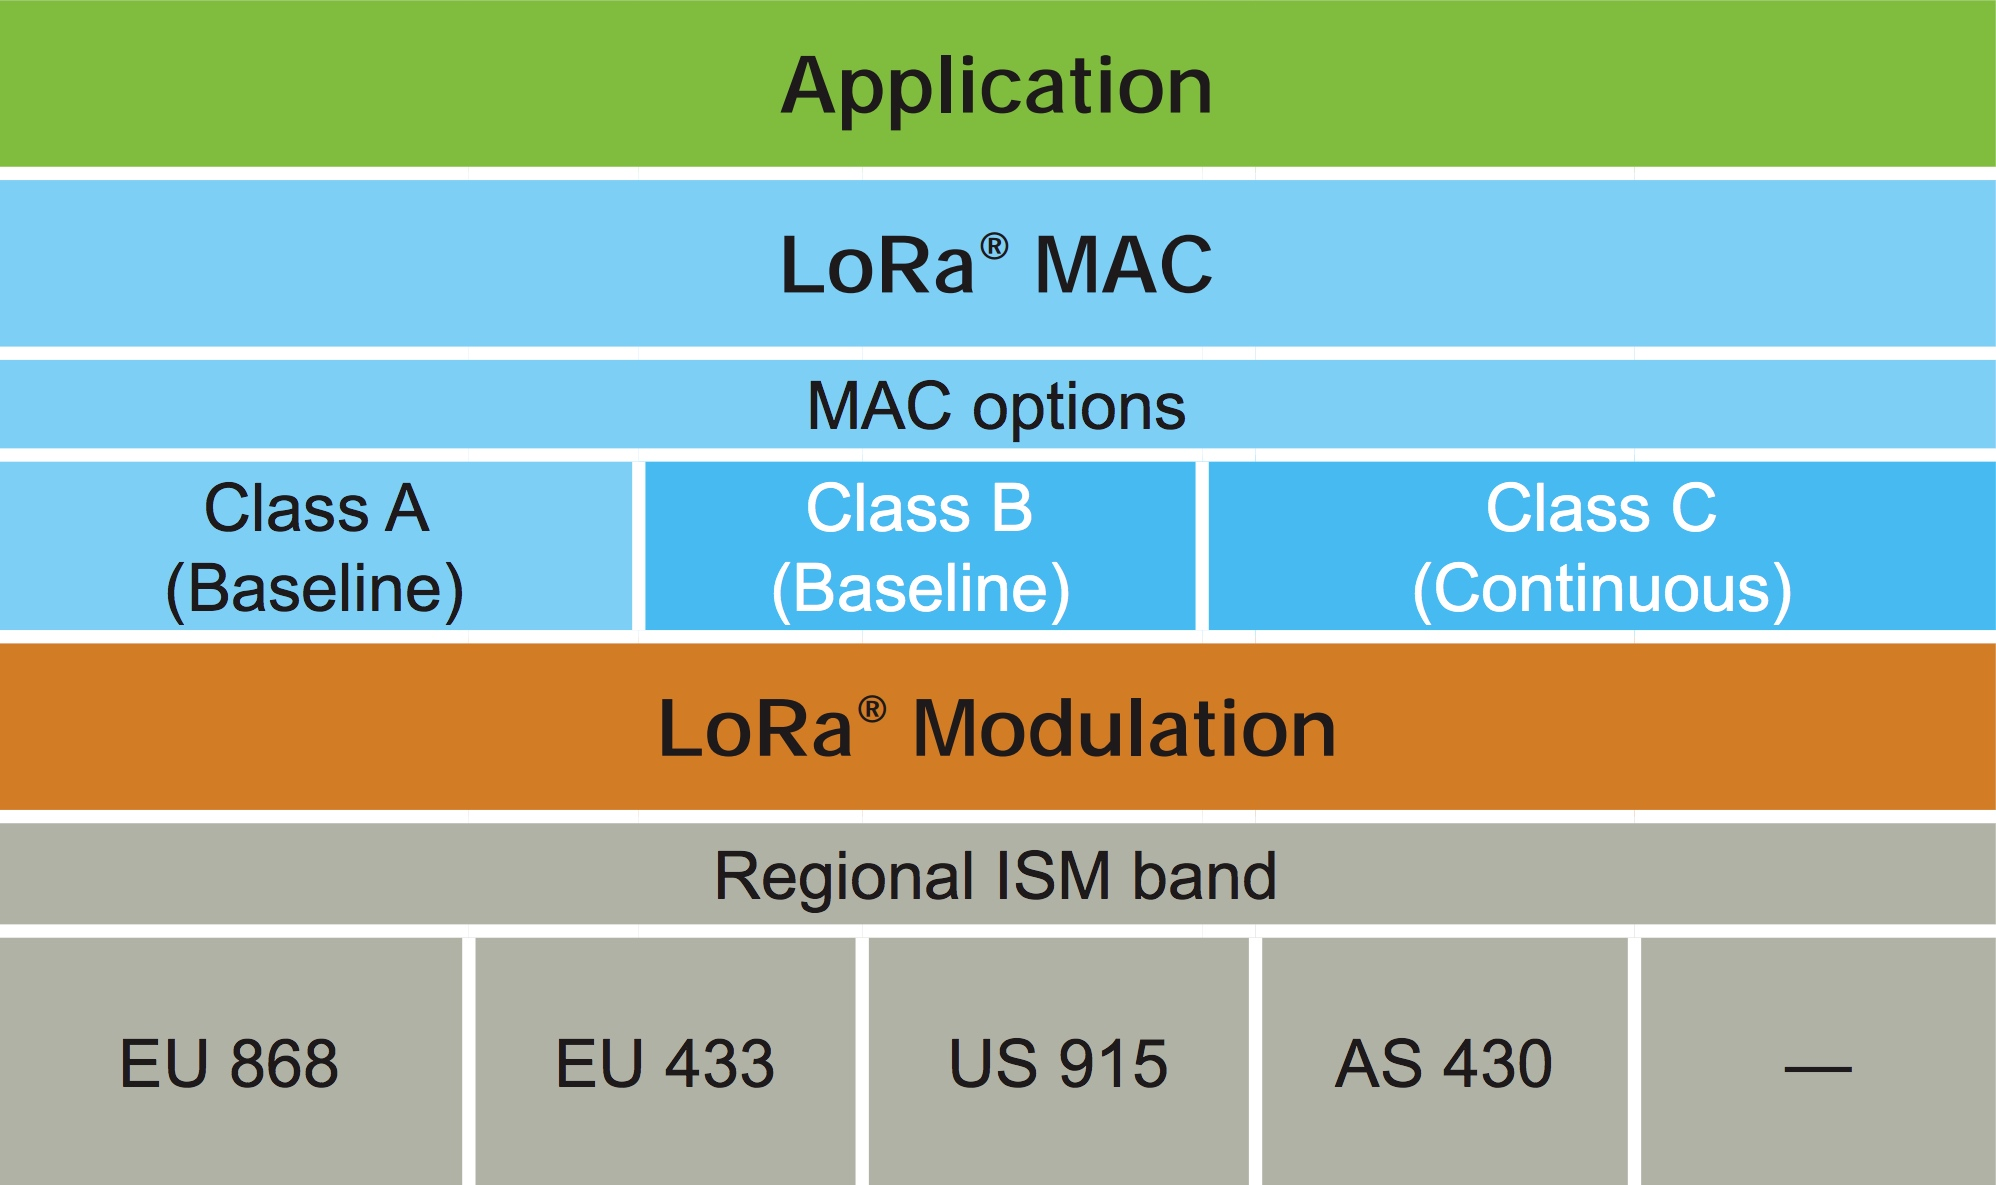
\includegraphics[width=1.0\textwidth]{pictures/lorawan-architecture.jpg}
    \caption{LoRaWAN Architektur}
    \label{fig:LoRaWAN Architektur}
\end{figure}

Viele bestehende Netzwerke verwenden eine Mesh-Netzwerk Architektur. In einem Mesh-Netzwerk leiten die einzelnen \gls{iotk} die Information an andere Knoten weiter um die Reichweite und Zellengrösse des Netzwerks zu vergrössern. Während dies die Reichweite verbessert, nimmt auch die Komplexität zu, reduziert die Netzwerkkapazität und verkürzt die Batterielaufzeit, da die Knoten Daten von anderen Knoten empfangen und weiterleiten, die für sie selber irrelevant ist. Eine auf weite Distanzen ausgelegte Stern-Architektur macht am meisten Sinn um die Batterielaufzeit hoch zu halten wenn dafür Verbindungen über lange Distanzen erreicht werden können. Aus diesem Grunde wurde \gls{lorawan} nicht auf die Mesh-Topologie aufgebaut. Die Kommunikation der Knoten in \gls{lorawan} ist asynchron, sie senden nur Daten wenn welche verfügbar sind, sei es ereignisbasiert oder in gewissen zeitlichen Abständen. Diese Art von Protokoll wird typischerweise als Aloha-Methode bezeichnet.

\subsubsection*{Netzwerk Architektur}

In einem \gls{lorawan} Netzwerk sind die \gls{iotk} nicht einem spezifischen Gateway zugeordnet. Stattdessen werden die von einem \gls{iotk} übermittelten Daten von mehreren Gateways empfangen. Jedes Gateway sendet diese Daten weiter zu einem zentralen Server (in Abbildung 5.2 Network Server genannt). Die Intelligenz und Komplexität wird auf diesen Server verschoben. Er übernimmt das Deduplizieren von redundanten Paketen, überprüft die Sicherheit, legt die Empfangsbestätigung über den optimalen Gateway fest und weist den \gls{iotk} adaptiv die beste Datenrate zu. Wenn ein Knoten mobil ist oder sich ständig bewegt ist kein Handover von Gateway zu Gateway nötig, was eine wichtige Anforderung ist, um beispielsweise bewegte Güter zu überwachen.

\begin{figure}[H]
     \centering
        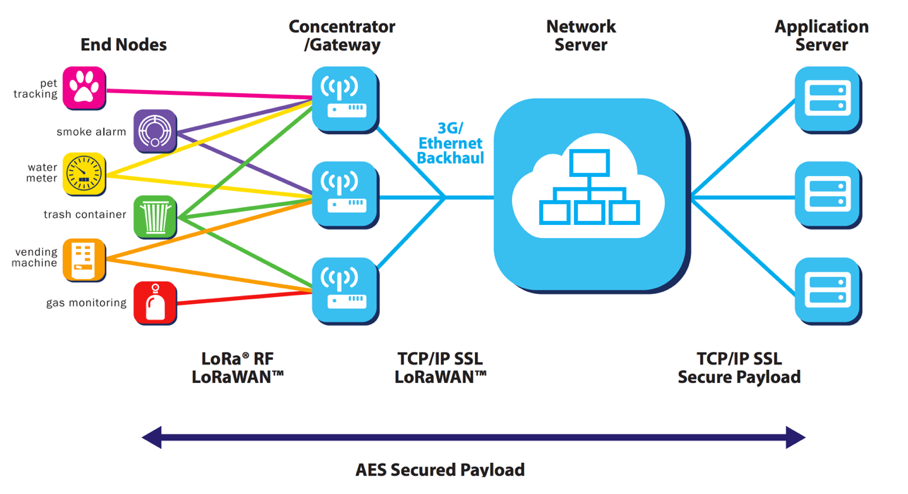
\includegraphics[width=1.0\textwidth]{pictures/lorawan-network-architecture.png}
    \caption{LoRaWAN Netzwerk Architektur}
    \label{fig:LoRaWAN Netzwerk Architektur}
\end{figure}

\subsubsection*{Netzwerkkapazität}

Je grösser der Einzugsraum eines \gls{iotg} ist, desto mehr Traffic muss dieser potentiell bewältigen. Da \gls{lorawan} auf grosse Reichweiten ausgelegt ist, muss es auch ein Konzept für hohe Netzwerkkapazitäten liefern. Dies macht \gls{lorawan} durch die Verwendung von adaptiven Datenraten und mit Multikanal- und Multimodem Transceivern. Das bedeutet, dass gleichzeitig Pakete auf mehreren Kanälen empfangen werden können. Die kritischen Faktoren, die die Kapazität betreffen, sind die Anzahl simultaner Kanäle, Datenrate (Zeit in der Luft), die Payload-Länge und wie häufig die Knoten Daten versenden. Dank der Frequenzspreizungsmodulation von \gls{lora}, stehen die Signale praktisch orthogonal zueinander, unter der Bedingung, dass unterschiedliche Spreizfaktoren verwendet werden. Wenn der Spreizfaktor ändert, ändert auch die effektive Datenrate. Ein Gateway nutzt diese Eigenschafte zu seinem Vorteil, indem er mehrere unterschiedliche Datenraten auf dem gleichen Kanal zur gleichen Zeit empfangen kann. Knoten mit guter Verbindung zum Gateway nutzen hohe Datenraten, um möglichst wenig Übertragungszeit zu verursachen und so die Luft möglichst lange frei zu lassen. Dies ergibt mehr potentiellen Platz für andere Pakete. Die adaptive Datenrate verlängert auch die Batterielaufzeit eines Knotens, da ihre Optimierung mehr freie Zeit in der Luft zur Verfügung stellt und somit Kollisionen verhindert werden können. Um eine adaptive Datenrate zu ermöglichen wird ein symmetrischer Up- und Downlink mit genügend Downlink Kapazität benötigt. Diese Merkmale ermöglichen einem \gls{lorawan} Netzwerk eine sehr Netzwerkkapazität, trotz beschränkter Datenraten im Sub-1Ghz Frequenzbereich. Die Adaptive Datenrate macht das Netzwerk zudem skalierbar, da dadurch die Verbindungen zwischen Knoten und Gateways optimiert werden. Ein Netzwerk kann mit minimaler Infrastruktur einfach aufgebaut werden und wenn mehr Kapazität benötigt wird können einfach mehr Gateways hinzugefügt werden. Dies erhöht die Datenraten, reduziert das Übersprechen auf andere Gateways und die Kapazität skaliert damit 6 bis 8 mal. Alternative \gls{lpwan} Technologien bieten nicht diese Skalierbarkeit, meistens weil sie die Downlink Kapazität einschränken oder das Verhältnis zwischen Up- und Downlink asymmetrisch machen.

\subsubsection*{Geräteklassen}

Endgeräte müssen verschiedene Aufgaben erfüllen und haben unterschiedliche Anforderungen. Um dieser Vielfalt von Anwendungsprofilen gerecht zu werden, sind in \gls{lorawan} drei verschiedene Geräteklassen definiert. Diese unterscheiden sich zwischen Reaktionszeit (vom Server zum \gls{iotk}) und dem Energieverbrauch der Endgeräte. In einer regel- oder aktorbasierten Anwendung ist die Reaktionszeit wichtig. Für \gls{iotk}, die nur sporadisch Sensordaten an den Server übermitteln, ist die Batterielaufzeit viel wichtiger. Folgende Geräteklassen existieren:

\textbf{Klasse A:} Endgeräte der Klasse A erlauben eine bidirektionale Kommunikation. Auf die Uplink Übertragung jedes Endgeräts folgen zwei kurze Downlink Empfangsfenster. Der Übertragungszeitpunkt wird je nach seinen Bedürfnissen vom Endgerät gesteuert. Er kann eine kleine zufällige Wartezeit definieren (ALOHA-Typ Protokoll) um Kollisionen zu verhindern. Die Klasse A Operation ist die energieeffizienteste für Endgeräte, welche nur Downlink Kommunikation mit dem Server, kurz nach jedem Übermitteln der Daten benötigen. Die Downlink Kommunikation vom Server muss zu jeder anderen Zeit bis zur nächsten geplanten Uplink Übertragung warten.

\textbf{Klasse B:} Endgeräte mit bidirektionaler Kommunikation und festgesetzten Empfangszeitfenstern. Zusätzlich zu zufälligen Empfangsfenstern der Klasse A, öffnen Klasse B Endgeräte weitere Empfangsfenster zu festgelegten Zeitpunkten. Damit Endgeräte wissen, wann sie ihr Empfangsfenster öffnen sollen, erhalten sie ein Zeit-Beacon vom Gateway zur Synchronisation. Dies erlaubt dem Server herauszufinden ob sich das Endgerät im Empfangszustand befindet.

\textbf{Klasse C:} Endgeräte mit bidirektionaler Kommunikation und maximalen Empfangsfenstern. Endgeräte der Klasse C haben fast kontinuierliche offene Zeitfenster. Sie sind nur geschlossen, wenn das Endgerät Daten überträgt oder ausgeschaltet ist.

\begin{figure}[H]
     \centering
        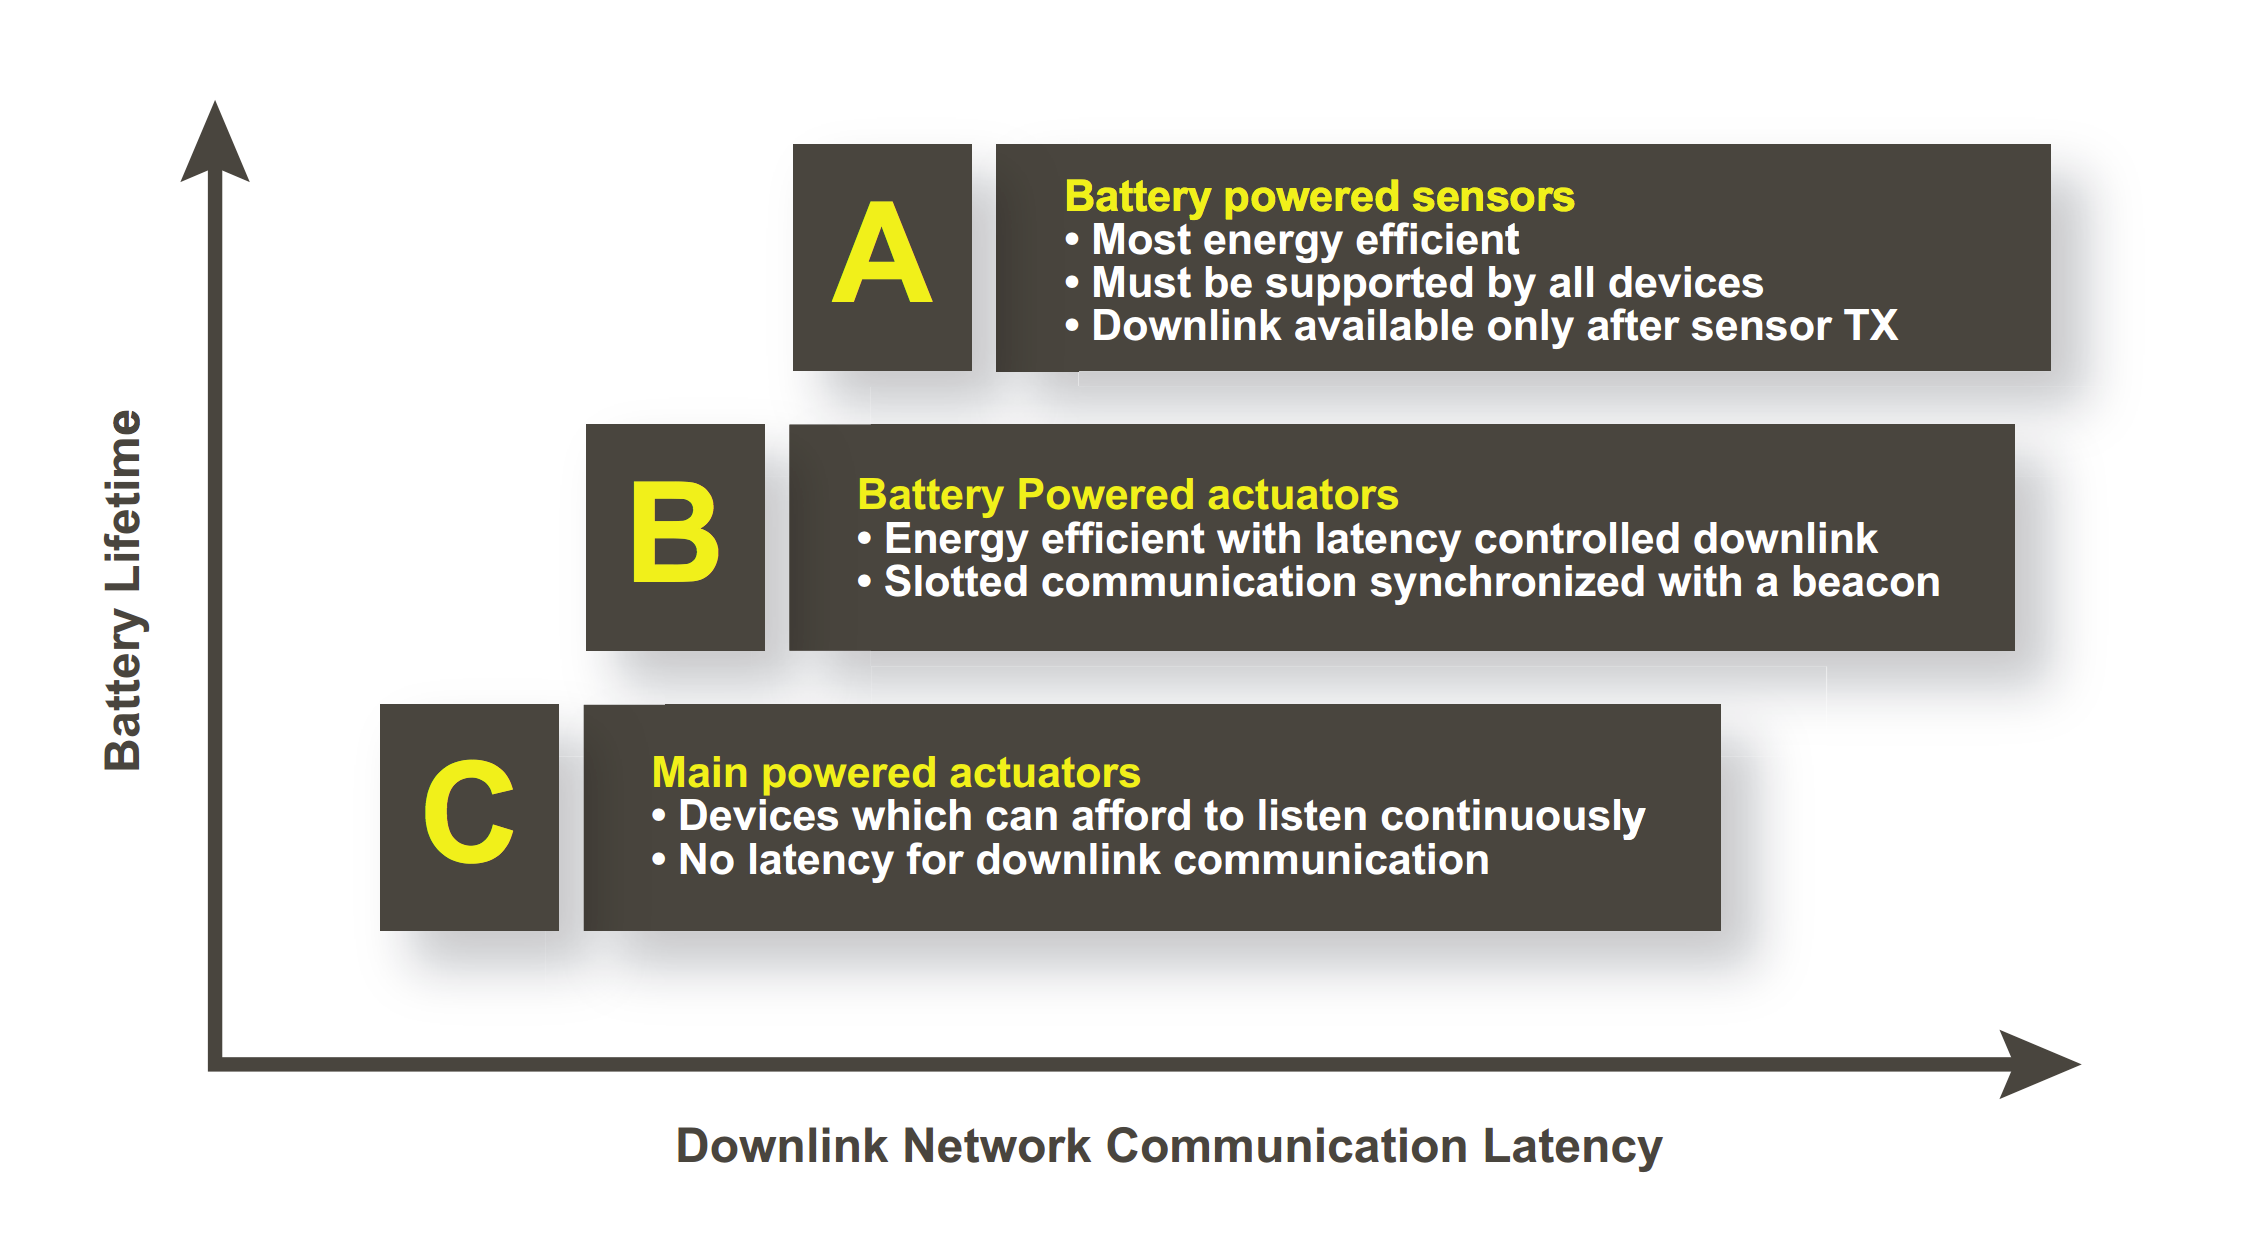
\includegraphics[width=0.9\textwidth]{pictures/device-classes.png}
    \caption{LoRaWAN Geräteklassen}
    \label{fig:LoRaWAN Geräteklassen}
\end{figure}

\begin{landscape}

\begin{table}[H]
\centering
% A table with adjusted row and column spacings
% \setlength sets the horizontal (column) spacing
% \arraystretch sets the vertical (row) spacing
\begingroup
\setlength{\tabcolsep}{10pt} % Default value: 6pt
\renewcommand{\arraystretch}{1.5} % Default value: 1
\begin{tabulary}{\paperwidth}{m{3cm} m{2cm} m{4cm} m{4cm} C m{2cm}}

\textbf{Modell}            & \textbf{Protokoll}                & \textbf{Frequenz}                                                                                        & \textbf{txPower}                                                               & \textbf{Sensivität} & \textbf{Reichweite}               \\ \hline
XBee-802.15.4-Pro          & 802.15.4                          & 2.4GHz                                                                                                   & 100mW                                                                          & -100dBm             & 7000m                             \\
XBee-ZB-Pro                & ZigBee-Pro                        & 2.4GHz                                                                                                   & 50mW                                                                           & -102dBm             & 7000m                             \\
XBee-868                   & RF                                & 868MHz                                                                                                   & 315mW                                                                          & -112dBm             & 12km                              \\
XBee-900                   & RF                                & 900MHz                                                                                                   & 50mW                                                                           & -100dBm             & 10Km                              \\
LoRaWAN                    & LoRaWAN                           & 868 and 433MHz. 900- 915MHz version coming in 2016.                                                      & 14dBm                                                                          & -136dBm             & - km - Typical base station range \\
LoRa                       & RF                                & 868 and 915 MHz                                                                                          & 14 dBm                                                                         & -137dBm             & 21+Km                             \\
Sigfox                     & Sigfox                            & 868MHz                                                                                                   & 14 dBm                                                                         & -126dBm             & - km - Typical base station range \\
WiFi                       & 802.11b/g                         & 2.4GHz                                                                                                   & 0dBm - 12dBm                                                                   & -83dBm              & 50m-500m                          \\
GPRS Pro and GPRS+GPS      & -                                 & 850MHz/900MHz/ 1800MHz/1900MHz                                                                           & 2W(Class4) 850MHz/900MHz, 1W(Class1) 1800MHz/1900MHz                           & -109dBm             & - Km - Typical carrier range      \\
3G/GPRS                    & -                                 & Tri-Band UMTS 2100/1900/900MHz Quad-Band GSM/EDGE, 850/900/1800/1900 MHz                                 & UMTS 900/1900/2100 0,25W GSM 850MHz/900MHz 2W DCS1800MHz/PCS1900MHz 1W         & -106dBm             & - Km - Typical carrier range      \\
Bluetooth Low Energy       & Bluetooth v.4.0 / Bluetooth Smart & 2.4GHz                                                                                                   & 3dBm                                                                           & -103dBm             & 100m
\end{tabulary}
\endgroup
% The \begingroup ... \endgroup pair ensures the separation
% parameters only affect this particular table, and not any
% sebsequent ones in the document.
\caption{RF-Technologien\autocite[18]{lora:TechGuide}}
\label{fig:IoT RF-Technologien}
\end{table}

\end{landscape}